\documentclass[twoside]{book}

% Packages required by doxygen
\usepackage{fixltx2e}
\usepackage{calc}
\usepackage{doxygen}
\usepackage[export]{adjustbox} % also loads graphicx
\usepackage{graphicx}
\usepackage[utf8]{inputenc}
\usepackage{makeidx}
\usepackage{multicol}
\usepackage{multirow}
\PassOptionsToPackage{warn}{textcomp}
\usepackage{textcomp}
\usepackage[nointegrals]{wasysym}
\usepackage[table]{xcolor}

% Font selection
\usepackage[T1]{fontenc}
\usepackage[scaled=.90]{helvet}
\usepackage{courier}
\usepackage{amssymb}
\usepackage{sectsty}
\renewcommand{\familydefault}{\sfdefault}
\allsectionsfont{%
  \fontseries{bc}\selectfont%
  \color{darkgray}%
}
\renewcommand{\DoxyLabelFont}{%
  \fontseries{bc}\selectfont%
  \color{darkgray}%
}
\newcommand{\+}{\discretionary{\mbox{\scriptsize$\hookleftarrow$}}{}{}}

% Page & text layout
\usepackage{geometry}
\geometry{%
  a4paper,%
  top=2.5cm,%
  bottom=2.5cm,%
  left=2.5cm,%
  right=2.5cm%
}
\tolerance=750
\hfuzz=15pt
\hbadness=750
\setlength{\emergencystretch}{15pt}
\setlength{\parindent}{0cm}
\setlength{\parskip}{3ex plus 2ex minus 2ex}
\makeatletter
\renewcommand{\paragraph}{%
  \@startsection{paragraph}{4}{0ex}{-1.0ex}{1.0ex}{%
    \normalfont\normalsize\bfseries\SS@parafont%
  }%
}
\renewcommand{\subparagraph}{%
  \@startsection{subparagraph}{5}{0ex}{-1.0ex}{1.0ex}{%
    \normalfont\normalsize\bfseries\SS@subparafont%
  }%
}
\makeatother

% Headers & footers
\usepackage{fancyhdr}
\pagestyle{fancyplain}
\fancyhead[LE]{\fancyplain{}{\bfseries\thepage}}
\fancyhead[CE]{\fancyplain{}{}}
\fancyhead[RE]{\fancyplain{}{\bfseries\leftmark}}
\fancyhead[LO]{\fancyplain{}{\bfseries\rightmark}}
\fancyhead[CO]{\fancyplain{}{}}
\fancyhead[RO]{\fancyplain{}{\bfseries\thepage}}
\fancyfoot[LE]{\fancyplain{}{}}
\fancyfoot[CE]{\fancyplain{}{}}
\fancyfoot[RE]{\fancyplain{}{\bfseries\scriptsize Generated by Doxygen }}
\fancyfoot[LO]{\fancyplain{}{\bfseries\scriptsize Generated by Doxygen }}
\fancyfoot[CO]{\fancyplain{}{}}
\fancyfoot[RO]{\fancyplain{}{}}
\renewcommand{\footrulewidth}{0.4pt}
\renewcommand{\chaptermark}[1]{%
  \markboth{#1}{}%
}
\renewcommand{\sectionmark}[1]{%
  \markright{\thesection\ #1}%
}

% Indices & bibliography
\usepackage{natbib}
\usepackage[titles]{tocloft}
\setcounter{tocdepth}{3}
\setcounter{secnumdepth}{5}
\makeindex

% Hyperlinks (required, but should be loaded last)
\usepackage{ifpdf}
\ifpdf
  \usepackage[pdftex,pagebackref=true]{hyperref}
\else
  \usepackage[ps2pdf,pagebackref=true]{hyperref}
\fi
\hypersetup{%
  colorlinks=true,%
  linkcolor=blue,%
  citecolor=blue,%
  unicode%
}

% Custom commands
\newcommand{\clearemptydoublepage}{%
  \newpage{\pagestyle{empty}\cleardoublepage}%
}

\usepackage{caption}
\captionsetup{labelsep=space,justification=centering,font={bf},singlelinecheck=off,skip=4pt,position=top}

%===== C O N T E N T S =====

\begin{document}

% Titlepage & ToC
\hypersetup{pageanchor=false,
             bookmarksnumbered=true,
             pdfencoding=unicode
            }
\pagenumbering{alph}
\begin{titlepage}
\vspace*{7cm}
\begin{center}%
{\Large Calculator }\\
\vspace*{1cm}
{\large Generated by Doxygen 1.8.13}\\
\end{center}
\end{titlepage}
\clearemptydoublepage
\pagenumbering{roman}
\tableofcontents
\clearemptydoublepage
\pagenumbering{arabic}
\hypersetup{pageanchor=true}

%--- Begin generated contents ---
\chapter{File Index}
\section{File List}
Here is a list of all documented files with brief descriptions\+:\begin{DoxyCompactList}
\item\contentsline{section}{src/\hyperlink{Calculator_8c}{Calculator.\+c} }{\pageref{Calculator_8c}}{}
\item\contentsline{section}{src/\hyperlink{main_8c}{main.\+c} }{\pageref{main_8c}}{}
\item\contentsline{section}{src/\hyperlink{User__interface_8c}{User\+\_\+interface.\+c} \\*This file is for anyone learning c programming Description \+: in this file we implement the function definition in which we get user inputs and ask him for operation then print the result }{\pageref{User__interface_8c}}{}
\end{DoxyCompactList}

\chapter{File Documentation}
\hypertarget{Calculator_8c}{}\section{src/\+Calculator.c File Reference}
\label{Calculator_8c}\index{src/\+Calculator.\+c@{src/\+Calculator.\+c}}
{\ttfamily \#include \char`\"{}../include/\+Calculator.\+h\char`\"{}}\newline
Include dependency graph for Calculator.\+c\+:
\nopagebreak
\begin{figure}[H]
\begin{center}
\leavevmode
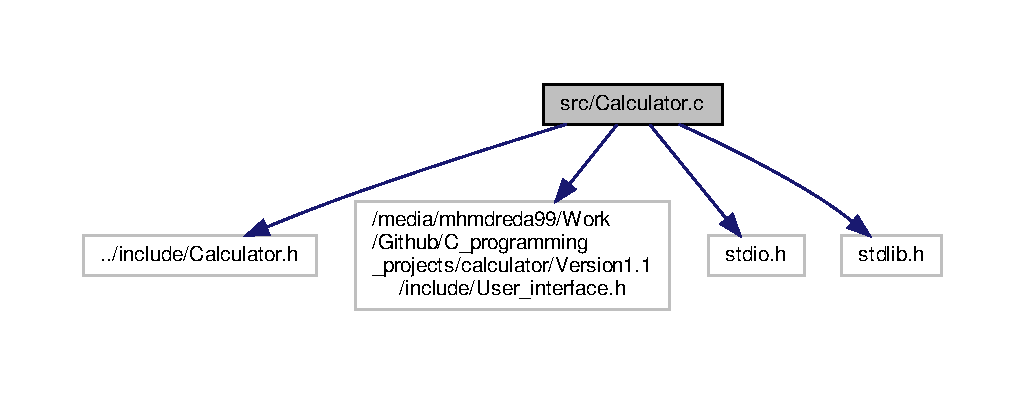
\includegraphics[width=350pt]{Calculator_8c__incl}
\end{center}
\end{figure}
\subsection*{Functions}
\begin{DoxyCompactItemize}
\item 
\mbox{\Hypertarget{Calculator_8c_ad8371d4d2d88050419cc73590a7c8244}\label{Calculator_8c_ad8371d4d2d88050419cc73590a7c8244}} 
void {\bfseries Calc\+\_\+\+App} (void)
\end{DoxyCompactItemize}


\subsection{Detailed Description}
\begin{DoxyAuthor}{Author}
mhmdreda99 (\href{mailto:Moreda491999@gmail.com}{\tt Moreda491999@gmail.\+com}) 
\end{DoxyAuthor}
\begin{DoxyVersion}{Version}
1.\+1 
\end{DoxyVersion}
\begin{DoxyDate}{Date}
2020-\/12-\/28
\end{DoxyDate}
\begin{DoxyCopyright}{Copyright}
Copyright (c) 2020 
\end{DoxyCopyright}

\hypertarget{main_8c}{}\section{src/main.c File Reference}
\label{main_8c}\index{src/main.\+c@{src/main.\+c}}
{\ttfamily \#include \char`\"{}../include/\+Calculator.\+h\char`\"{}}\newline
Include dependency graph for main.\+c\+:
\nopagebreak
\begin{figure}[H]
\begin{center}
\leavevmode
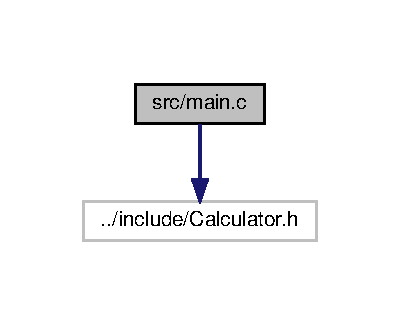
\includegraphics[width=192pt]{main_8c__incl}
\end{center}
\end{figure}
\subsection*{Functions}
\begin{DoxyCompactItemize}
\item 
int \hyperlink{main_8c_ae66f6b31b5ad750f1fe042a706a4e3d4}{main} ()
\begin{DoxyCompactList}\small\item\em we just call main application fro other files \end{DoxyCompactList}\end{DoxyCompactItemize}


\subsection{Detailed Description}
\begin{DoxyAuthor}{Author}
Moahmed reda 
\end{DoxyAuthor}
\begin{DoxyVersion}{Version}
1.\+1 
\end{DoxyVersion}
\begin{DoxyDate}{Date}
2020-\/12-\/28
\end{DoxyDate}
\begin{DoxyCopyright}{Copyright}
Copyright (c) 2020 
\end{DoxyCopyright}


\subsection{Function Documentation}
\mbox{\Hypertarget{main_8c_ae66f6b31b5ad750f1fe042a706a4e3d4}\label{main_8c_ae66f6b31b5ad750f1fe042a706a4e3d4}} 
\index{main.\+c@{main.\+c}!main@{main}}
\index{main@{main}!main.\+c@{main.\+c}}
\subsubsection{\texorpdfstring{main()}{main()}}
{\footnotesize\ttfamily int main (\begin{DoxyParamCaption}{ }\end{DoxyParamCaption})}



we just call main application fro other files 

\begin{DoxyReturn}{Returns}
int for ending program 
\end{DoxyReturn}

\hypertarget{User__interface_8c}{}\section{src/\+User\+\_\+interface.c File Reference}
\label{User__interface_8c}\index{src/\+User\+\_\+interface.\+c@{src/\+User\+\_\+interface.\+c}}


this file is for anyone learning c programming Description \+: in this file we implement the function definition in which we get user inputs and ask him for operation then print the result  


{\ttfamily \#include \char`\"{}../include/\+User\+\_\+interface.\+h\char`\"{}}\newline
Include dependency graph for User\+\_\+interface.\+c\+:
\nopagebreak
\begin{figure}[H]
\begin{center}
\leavevmode
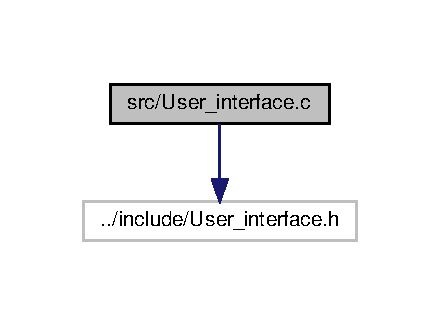
\includegraphics[width=211pt]{User__interface_8c__incl}
\end{center}
\end{figure}
\subsection*{Functions}
\begin{DoxyCompactItemize}
\item 
\mbox{\Hypertarget{User__interface_8c_a5706cf39829372a25ff9106ed5ae9c57}\label{User__interface_8c_a5706cf39829372a25ff9106ed5ae9c57}} 
void \hyperlink{User__interface_8c_a5706cf39829372a25ff9106ed5ae9c57}{User\+\_\+\+Interface} (void)
\begin{DoxyCompactList}\small\item\em this is a printing func. that displays the following massages on screen \end{DoxyCompactList}\item 
\mbox{\Hypertarget{User__interface_8c_ad3a8d669a31bd808c504ed7608662350}\label{User__interface_8c_ad3a8d669a31bd808c504ed7608662350}} 
void \hyperlink{User__interface_8c_ad3a8d669a31bd808c504ed7608662350}{Get\+\_\+\+User\+\_\+\+Input} (void)
\begin{DoxyCompactList}\small\item\em ask user to choose the operation by enter the operation char.(+,$\ast$,-\/,/) and simply get user input and store the two numbers in num1,num2 \end{DoxyCompactList}\item 
\mbox{\Hypertarget{User__interface_8c_a22c7427ff20328ee4e807abebba08031}\label{User__interface_8c_a22c7427ff20328ee4e807abebba08031}} 
void \hyperlink{User__interface_8c_a22c7427ff20328ee4e807abebba08031}{Print\+\_\+\+Result} (void)
\begin{DoxyCompactList}\small\item\em printing result on the screen \end{DoxyCompactList}\end{DoxyCompactItemize}
\subsection*{Variables}
\begin{DoxyCompactItemize}
\item 
\mbox{\Hypertarget{User__interface_8c_a00e5a73548232a9da31fb2bf0df308c1}\label{User__interface_8c_a00e5a73548232a9da31fb2bf0df308c1}} 
float {\bfseries num1}
\item 
\mbox{\Hypertarget{User__interface_8c_adec9cc9604b26a053295a65b16b8f746}\label{User__interface_8c_adec9cc9604b26a053295a65b16b8f746}} 
float {\bfseries num2}
\item 
\mbox{\Hypertarget{User__interface_8c_a8b6cc3f78b62c5c59645624670120e4d}\label{User__interface_8c_a8b6cc3f78b62c5c59645624670120e4d}} 
float {\bfseries result}
\item 
\mbox{\Hypertarget{User__interface_8c_a454fa9de3ca009e3082488412cd184d4}\label{User__interface_8c_a454fa9de3ca009e3082488412cd184d4}} 
char {\bfseries option}
\end{DoxyCompactItemize}


\subsection{Detailed Description}
this file is for anyone learning c programming Description \+: in this file we implement the function definition in which we get user inputs and ask him for operation then print the result 

\begin{DoxyAuthor}{Author}
mhmdreda99 (\href{mailto:Moreda491999@gmail.com}{\tt Moreda491999@gmail.\+com}) 
\end{DoxyAuthor}
\begin{DoxyVersion}{Version}
1.\+1 
\end{DoxyVersion}
\begin{DoxyDate}{Date}
2020-\/12-\/28
\end{DoxyDate}
\begin{DoxyCopyright}{Copyright}
Copyright (c) 2020 
\end{DoxyCopyright}

%--- End generated contents ---

% Index
\backmatter
\newpage
\phantomsection
\clearemptydoublepage
\addcontentsline{toc}{chapter}{Index}
\printindex

\end{document}
